%%%%%%%%%%%%%%%%%%%%%%%%%%%%%%%%%%%%%%%%%%%%%%%%%%%%%%%%%%%%%%%%%%%%%%%%%%%%%%%%
\subsection{Πειραματική διαδικασία}
\label{subsection:02_02_04:01}

Το περιεχόμενο της παρούσας ενότητας εξυπηρετεί τον έλεγχο τριών διακριτών
υποθέσεων, όπως αρθρώθηκαν στις ενότητες \ref{subsection:02_02_03:01},
\ref{subsection:02_02_03:02}, και \ref{subsection:02_02_03:03}:

\begin{enumerate}
  \item[(H1)] Η επιλογή σωματιδίων υψηλού βάρους από τον πληθυσμό του
        MCL---ισοδύναμα: η απόρριψη σωματιδίων χαμηλού βάρους από αυτόν---και o
        υπολογισμός της εκτίμησης του φίλτρου ως ο σταθμισμένος μέσος όρος
        των στάσεων τους έχει ως αποτέλεσμα αυξημένη ακρίβεια στάσης σε σύγκριση
        με την επιλογή όλων των σωματιδίων από τον πληθυσμό
  \item[(H2)] Η ευθυγράμμιση μεταξύ α) μιας μέτρησης που λαμβάνεται μέσω του
        φυσικού αισθητήρα lidar του ρομπότ από την πραγματική του στάση και
        (β) μιας εικονικής σάρωσης που λαμβάνεται εντός του χάρτη στον οποίο
        πλοηγείται το ρομπότ από την εκτιμώμενη στάση του αισθητήρα, και η
        εφαρμογή του προκύπτοντος μετασχηματισμού στην εκτίμηση της στάσης του
        MCL έχει ως αποτέλεσμα αυξημένη ακρίβεια στάσης σε σύγκριση με τον MCL
        απουσία ανατροφοδότησης
  \item[(H3)] Η ανατροφοδότηση της (υποθετικά βελτιωμένης) στάσης στον πληθυσμό
        του MCL με τη μορφή μιας ομάδας σωματιδίων που αποτελούν το $p\%$ του
        τελικού πληθυσμού σωματιδίων, όπου $p$ είναι αρκετά μικρότερο από $100$
        και αρκετά μεγαλύτερο από $1$, (α) έχει ως αποτέλεσμα αυξημένη ακρίβεια
        στάσης σε σύγκριση με τον MCL, (β) έχει ως αποτέλεσμα αυξημένη ακρίβεια
        στάσης σε σύγκριση με την ανατροφοδότηση μόνο ενός σωματιδίου με την εν
        λόγω διορθωμένη στάση, και (γ) είναι πιο εύρωστη από την εκ νέου
        αρχικοποίηση του MCL γύρω από τη μετασχηματισμένη στάση
\end{enumerate}

Στην τρίτη υπόθεση αναφερόμαστε στην ευρωστία με την έννοια της ικανότητας ενός
συστήματος να αποφεύγει την αποτυχία και όχι να ανακάμπτει από αυτήν, η οποία
ικανότητα αναφέρεται ως ``ανθεκτικότητα" (resilience)
\cite{Zhu2011b,Tavana2011}. Η ικανότητα ανάκαμψης από αποτυχίες είναι μια
ιδιότητα του ίδιου του φίλτρου σωματιδίων, ενώ η ικανότητα αποφυγής αποτυχίας
(στην προκειμένη περίπτωση η επανεκκίνηση γύρω από μία καταστροφικά λανθασμένη
στάση) είναι ιδιότητα της μεθόδου ανατροφοδότησης.

Οι υποθέσεις αυτές δοκιμάζονται σε δύο διακριτά προσομοιωμένα περιβάλλοντα. To
πρώτο περιβάλλον ονομάζεται CORRIDOR, συμβολίζεται με $\bm{M}_C$, και
παρουσιάζεται στο σχήμα \ref{fig:02_02_04:maps}(α'). Το δεύτερο ονομάζεται
WAREHOUSE, συμβολίζεται με $\bm{M}_W$, και παρουσιάζεται στο σχήμα
\ref{fig:02_02_04:maps}(β'). Η ανάλυση και των δύο χαρτών είναι $0.01$ m
$\times0.01$ m ανά κελί πλέγματος. Ο πρώτος χρησιμοποιείται για να δείξει την
αποτελεσματικότητα του προτεινόμενου συστήματος σε μη σύνθετα περιβάλλοντα,
όπου όλα τα όριά του βρίσκονται εντός της μέγιστης εμβέλειας του αισθητήρα
lidar του ρομπότ ανά πάσα στιγμή.  Αντίθετα, το δεύτερο είναι μια μεγάλη
αποθήκη, που προορίζεται να θέσει μεγαλύτερη πρόκληση στο σύστημα και συνεπώς
στην απόδοσή του: τα εμπόδια βρίσκονται σε μεγαλύτερη απόσταση μεταξύ τους από
ότι στο CORRIDOR, πράγμα που σημαίνει ότι είτε δεν φέρουν όλες οι ακτίνες του
αισθητήρα αξιοποιήσιμη πληροφορία, είτε αλλοιώνονται περισσότερο από θόρυβο,
καθώς το σφάλμα απόστασης αυξάνεται με την μετρήσιμη απόσταση, ή και τα δύο. Η
πρώτη πρόκληση επηρεάζει (α) τον MCL, καθώς πρέπει να βασίζεται περισσότερο
στην οδομετρία του, η οποία είναι επιρρεπής στη συσσώρευση σφαλμάτων, και
λιγότερο στις μετρήσεις απόστασης και (β) την ευθυγράμμιση σαρώσεων, καθώς
υπάρχουν λιγότερα μετρούμενα σημεία σάρωσης και άρα μεγαλύτερη ανεπάρκεια
πληροφοριών κατά την ευθυγράμμιση μετρήσεων με σαρώσεις. Η δεύτερη πρόκληση
επηρεάζει (α) τον MCL δεδομένου ότι η εκτίμηση της στάσης διαταράσσεται από
θόρυβο μέτρησης, και (β) την ευθυγράμμιση μετρήσεων με σαρώσεις, καθώς ο
θόρυβος αυξάνει την πιθανότητα λανθασμένων αντιστοιχίσεων και, γενικά, της
εσφαλμένης ευθυγράμμισης συνολικά. Για το σκοπό αυτό ρυθμίσαμε τον αισθητήρα
αποστάσεων ώστε να λειτουργεί με μέγιστη εμβέλεια $10.0$ μέτρα.  Σε όλες τις
προσομοιώσεις χρησιμοποιήθηκε ο MCL παράλληλα με τη δειγματοληψία KLD, με
ελάχιστο και μέγιστο αριθμό σωματιδίων $N_{\min}=200$ και $N_{\max}=500$.  Οι
τρεις ως άνω υποθέσεις δοκιμάζονται κατά τη διαδικασία αυτόνομης πλοήγησης στα
δύο ως άνω περιβάλλοντα. Οι αρχικές και τελικές στάσεις για κάθε χάρτη ήταν (α)
$\bm{M}_C$: $\bm{x}_0^{\bm{M}_C} \equiv (11.56\text{ m}, 12.20\text{ m}, 0.0
\text{ rad})$, και $\bm{x}_G^{\bm{M}_C} \equiv (5.0 \text{ m}, 6.0 \text{ m},
0.0 \text{ rad})$, αντίστοιχα, και (β) $\bm{M}_W$: $\bm{x}_0^{\bm{M}_W} \equiv
(17.98 \text{ m}, 2.08 \text{ m}, \pi/2 \text{ rad})$, και $\bm{x}_G^{\bm{M}_W}
\equiv (6.0 \text{ m}, 40.0 \text{ m}, \pi/2 \text{ rad})$ αντίστοιχα. Οι
αρχικές και οι τελικές στάσεις για κάθε χάρτη σχεδιάζονται με πράσινο και
κόκκινο χρώμα στα αντίστοιχα σχήματα.  Το ρομπότ που χρησιμοποιήθηκε κατά την
πειραματική διαδικασία είναι το Turtlebot v.2, εξοπλισμένο με αισθητήρα
απόστασης μέγιστης εμβέλειας $r_{max} = 10.0$ m, γωνιακού εύρους $\alpha =
260^{\circ}$, και αριθμό ακτίνων $N_s = 640$, του οποίου οι μετρήσεις
αλλοιώνονται από θόρυβο κανονικά κατανεμημένο, με μηδενική μέση τιμή και τυπική
απόκλιση $\sigma_R = 0.01$ m.

\begin{figure}\hspace{0.5cm}
  \begin{subfigure}{0.49\linewidth}\centering
    \vspace{1.0cm}
    \definecolor{r}{RGB}{255 0 0}
\definecolor{g}{RGB}{0 155 0}
% GNUPLOT: LaTeX picture with Postscript
\begingroup
  \makeatletter
  \providecommand\color[2][]{%
    \GenericError{(gnuplot) \space\space\space\@spaces}{%
      Package color not loaded in conjunction with
      terminal option `colourtext'%
    }{See the gnuplot documentation for explanation.%
    }{Either use 'blacktext' in gnuplot or load the package
      color.sty in LaTeX.}%
    \renewcommand\color[2][]{}%
  }%
  \providecommand\includegraphics[2][]{%
    \GenericError{(gnuplot) \space\space\space\@spaces}{%
      Package graphicx or graphics not loaded%
    }{See the gnuplot documentation for explanation.%
    }{The gnuplot epslatex terminal needs graphicx.sty or graphics.sty.}%
    \renewcommand\includegraphics[2][]{}%
  }%
  \providecommand\rotatebox[2]{#2}%
  \@ifundefined{ifGPcolor}{%
    \newif\ifGPcolor
    \GPcolorfalse
  }{}%
  \@ifundefined{ifGPblacktext}{%
    \newif\ifGPblacktext
    \GPblacktexttrue
  }{}%
  % define a \g@addto@macro without @ in the name:
  \let\gplgaddtomacro\g@addto@macro
  % define empty templates for all commands taking text:
  \gdef\gplfronttext{}%
  \gdef\gplfronttext{}%
  \makeatother
  \ifGPblacktext
    % no textcolor at all
    \def\colorrgb#1{}%
    \def\colorgray#1{}%
  \else
    % gray or color?
    \ifGPcolor
      \def\colorrgb#1{\color[rgb]{#1}}%
      \def\colorgray#1{\color[gray]{#1}}%
      \expandafter\def\csname LTw\endcsname{\color{white}}%
      \expandafter\def\csname LTb\endcsname{\color{black}}%
      \expandafter\def\csname LTa\endcsname{\color{black}}%
      \expandafter\def\csname LT0\endcsname{\color[rgb]{1,0,0}}%
      \expandafter\def\csname LT1\endcsname{\color[rgb]{0,1,0}}%
      \expandafter\def\csname LT2\endcsname{\color[rgb]{0,0,1}}%
      \expandafter\def\csname LT3\endcsname{\color[rgb]{1,0,1}}%
      \expandafter\def\csname LT4\endcsname{\color[rgb]{0,1,1}}%
      \expandafter\def\csname LT5\endcsname{\color[rgb]{1,1,0}}%
      \expandafter\def\csname LT6\endcsname{\color[rgb]{0,0,0}}%
      \expandafter\def\csname LT7\endcsname{\color[rgb]{1,0.3,0}}%
      \expandafter\def\csname LT8\endcsname{\color[rgb]{0.5,0.5,0.5}}%
    \else
      % gray
      \def\colorrgb#1{\color{black}}%
      \def\colorgray#1{\color[gray]{#1}}%
      \expandafter\def\csname LTw\endcsname{\color{white}}%
      \expandafter\def\csname LTb\endcsname{\color{black}}%
      \expandafter\def\csname LTa\endcsname{\color{black}}%
      \expandafter\def\csname LT0\endcsname{\color{black}}%
      \expandafter\def\csname LT1\endcsname{\color{black}}%
      \expandafter\def\csname LT2\endcsname{\color{black}}%
      \expandafter\def\csname LT3\endcsname{\color{black}}%
      \expandafter\def\csname LT4\endcsname{\color{black}}%
      \expandafter\def\csname LT5\endcsname{\color{black}}%
      \expandafter\def\csname LT6\endcsname{\color{black}}%
      \expandafter\def\csname LT7\endcsname{\color{black}}%
      \expandafter\def\csname LT8\endcsname{\color{black}}%
    \fi
  \fi
  \setlength{\unitlength}{0.03200bp}%
  \begin{picture}(4000.00,4000.00)%
    \gplgaddtomacro\gplfronttext{%
      \colorrgb{0.00,0.00,0.00}%
      \put(388,778){\makebox(0,0)[r]{\strut{} \footnotesize $4$}}%
      \colorrgb{0.00,0.00,0.00}%
      \put(388,1295){\makebox(0,0)[r]{\strut{}\footnotesize $6$}}%
      \colorrgb{0.00,0.00,0.00}%
      \put(388,1811){\makebox(0,0)[r]{\strut{}\footnotesize $8$}}%
      \colorrgb{0.00,0.00,0.00}%
      \put(388,2328){\makebox(0,0)[r]{\strut{}\footnotesize $10$}}%
      \colorrgb{0.00,0.00,0.00}%
      \put(388,2844){\makebox(0,0)[r]{\strut{}\footnotesize $12$}}%
      \colorrgb{0.00,0.00,0.00}%
      \put(388,3361){\makebox(0,0)[r]{\strut{}\footnotesize $14$}}%
      \colorrgb{0.00,0.00,0.00}%
      \put(778,300){\makebox(0,0){\strut{} \footnotesize $4$}}%
      \colorrgb{0.00,0.00,0.00}%
      \put(1295,300){\makebox(0,0){\strut{}\footnotesize $6$}}%
      \colorrgb{0.00,0.00,0.00}%
      \put(1811,300){\makebox(0,0){\strut{}\footnotesize $8$}}%
      \colorrgb{0.00,0.00,0.00}%
      \put(2328,300){\makebox(0,0){\strut{}\footnotesize $10$}}%
      \colorrgb{0.00,0.00,0.00}%
      \put(2844,300){\makebox(0,0){\strut{}\footnotesize $12$}}%
      \colorrgb{0.00,0.00,0.00}%
      \put(3361,300){\makebox(0,0){\strut{}\footnotesize $14$}}%
      \colorrgb{0.00,0.00,0.00}%
      \put(-118,2069){\rotatebox{90}{\makebox(0,0){\strut{}$y$ [m]}}}%
      \colorrgb{0.00,0.00,0.00}%
      \put(2069,-30){\makebox(0,0){\strut{}$x$ [m]}}%
      \put(2484,2784){\makebox(0,0){\strut{}\textcolor{g}{$\bm{p}_0$}}}%
      \put(1100,1600){\makebox(0,0){\strut{}\textcolor{r}{$\bm{p}_G$}}}%
    }%
    \gplgaddtomacro\gplfronttext{%
    }%
    \put(0,0){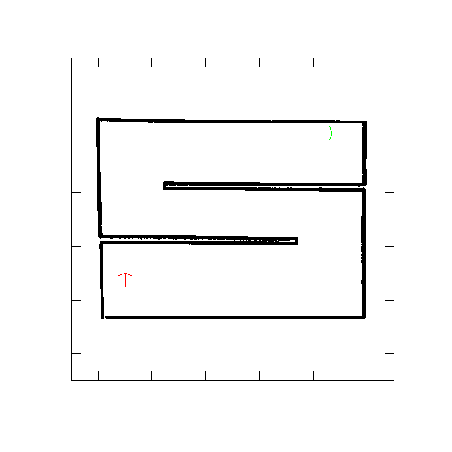
\includegraphics[scale=0.64]{./figures/slides/ch4/corridor}}%
    \gplfronttext
  \end{picture}%
\endgroup

    \vspace{1.0cm}
    \caption{\small Χάρτης του CORRIDOR, $\bm{M}_C$}
    \label{fig:02_02_04:map_corridor}
  \end{subfigure}\hfill
  \begin{subfigure}{0.49\linewidth} \centering
    \definecolor{r}{RGB}{255 0 0}
\definecolor{g}{RGB}{0 155 0}
% GNUPLOT: LaTeX picture with Postscript
\begingroup
  \makeatletter
  \providecommand\color[2][]{%
    \GenericError{(gnuplot) \space\space\space\@spaces}{%
      Package color not loaded in conjunction with
      terminal option `colourtext'%
    }{See the gnuplot documentation for explanation.%
    }{Either use 'blacktext' in gnuplot or load the package
      color.sty in LaTeX.}%
    \renewcommand\color[2][]{}%
  }%
  \providecommand\includegraphics[2][]{%
    \GenericError{(gnuplot) \space\space\space\@spaces}{%
      Package graphicx or graphics not loaded%
    }{See the gnuplot documentation for explanation.%
    }{The gnuplot epslatex terminal needs graphicx.sty or graphics.sty.}%
    \renewcommand\includegraphics[2][]{}%
  }%
  \providecommand\rotatebox[2]{#2}%
  \@ifundefined{ifGPcolor}{%
    \newif\ifGPcolor
    \GPcolorfalse
  }{}%
  \@ifundefined{ifGPblacktext}{%
    \newif\ifGPblacktext
    \GPblacktexttrue
  }{}%
  % define a \g@addto@macro without @ in the name:
  \let\gplgaddtomacro\g@addto@macro
  % define empty templates for all commands taking text:
  \gdef\gplfronttext{}%
  \gdef\gplfronttext{}%
  \makeatother
  \ifGPblacktext
    % no textcolor at all
    \def\colorrgb#1{}%
    \def\colorgray#1{}%
  \else
    % gray or color?
    \ifGPcolor
      \def\colorrgb#1{\color[rgb]{#1}}%
      \def\colorgray#1{\color[gray]{#1}}%
      \expandafter\def\csname LTw\endcsname{\color{white}}%
      \expandafter\def\csname LTb\endcsname{\color{black}}%
      \expandafter\def\csname LTa\endcsname{\color{black}}%
      \expandafter\def\csname LT0\endcsname{\color[rgb]{1,0,0}}%
      \expandafter\def\csname LT1\endcsname{\color[rgb]{0,1,0}}%
      \expandafter\def\csname LT2\endcsname{\color[rgb]{0,0,1}}%
      \expandafter\def\csname LT3\endcsname{\color[rgb]{1,0,1}}%
      \expandafter\def\csname LT4\endcsname{\color[rgb]{0,1,1}}%
      \expandafter\def\csname LT5\endcsname{\color[rgb]{1,1,0}}%
      \expandafter\def\csname LT6\endcsname{\color[rgb]{0,0,0}}%
      \expandafter\def\csname LT7\endcsname{\color[rgb]{1,0.3,0}}%
      \expandafter\def\csname LT8\endcsname{\color[rgb]{0.5,0.5,0.5}}%
    \else
      % gray
      \def\colorrgb#1{\color{black}}%
      \def\colorgray#1{\color[gray]{#1}}%
      \expandafter\def\csname LTw\endcsname{\color{white}}%
      \expandafter\def\csname LTb\endcsname{\color{black}}%
      \expandafter\def\csname LTa\endcsname{\color{black}}%
      \expandafter\def\csname LT0\endcsname{\color{black}}%
      \expandafter\def\csname LT1\endcsname{\color{black}}%
      \expandafter\def\csname LT2\endcsname{\color{black}}%
      \expandafter\def\csname LT3\endcsname{\color{black}}%
      \expandafter\def\csname LT4\endcsname{\color{black}}%
      \expandafter\def\csname LT5\endcsname{\color{black}}%
      \expandafter\def\csname LT6\endcsname{\color{black}}%
      \expandafter\def\csname LT7\endcsname{\color{black}}%
      \expandafter\def\csname LT8\endcsname{\color{black}}%
    \fi
  \fi
  \setlength{\unitlength}{0.03200bp}%
  \begin{picture}(4000.00,5000.00)%
    \gplgaddtomacro\gplfronttext{%
      \colorrgb{0.00,0.00,0.00}%
      \put(520,727){\makebox(0,0)[r]{\strut{} \footnotesize $0$}}%
      \colorrgb{0.00,0.00,0.00}%
      \put(520,1170){\makebox(0,0)[r]{\strut{}\footnotesize $5$}}%
      \colorrgb{0.00,0.00,0.00}%
      \put(520,1613){\makebox(0,0)[r]{\strut{}\footnotesize $10$}}%
      \colorrgb{0.00,0.00,0.00}%
      \put(520,2056){\makebox(0,0)[r]{\strut{}\footnotesize $15$}}%
      \colorrgb{0.00,0.00,0.00}%
      \put(520,2498){\makebox(0,0)[r]{\strut{}\footnotesize $20$}}%
      \colorrgb{0.00,0.00,0.00}%
      \put(520,2941){\makebox(0,0)[r]{\strut{}\footnotesize $25$}}%
      \colorrgb{0.00,0.00,0.00}%
      \put(520,3384){\makebox(0,0)[r]{\strut{}\footnotesize $30$}}%
      \colorrgb{0.00,0.00,0.00}%
      \put(520,3827){\makebox(0,0)[r]{\strut{}\footnotesize $35$}}%
      \colorrgb{0.00,0.00,0.00}%
      \put(520,4270){\makebox(0,0)[r]{\strut{}\footnotesize $40$}}%
      \colorrgb{0.00,0.00,0.00}%
      \put(1095,330){\makebox(0,0){\strut{}\footnotesize $0$}}%
      \colorrgb{0.00,0.00,0.00}%
      \put(1538,330){\makebox(0,0){\strut{}\footnotesize $5$}}%
      \colorrgb{0.00,0.00,0.00}%
      \put(1980,330){\makebox(0,0){\strut{}\footnotesize $10$}}%
      \colorrgb{0.00,0.00,0.00}%
      \put(2423,330){\makebox(0,0){\strut{}\footnotesize $15$}}%
      \colorrgb{0.00,0.00,0.00}%
      \put(2866,330){\makebox(0,0){\strut{}\footnotesize $20$}}%
      \colorrgb{0.00,0.00,0.00}%
      \put(-94,2587){\rotatebox{90}{\makebox(0,0){\strut{}$y$ [m]}}}%
      \colorrgb{0.00,0.00,0.00}%
      \put(2069,0){\makebox(0,0){\strut{}$x$ [m]}}%
      \put(2750,1300){\makebox(0,0){\strut{}\textcolor{g}{$\bm{p}_0$}}}%
      \put(2000,4300){\makebox(0,0){\strut{}\textcolor{r}{$\bm{p}_G$}}}%
    }%
    \gplgaddtomacro\gplfronttext{%
    }%
    \put(0,0){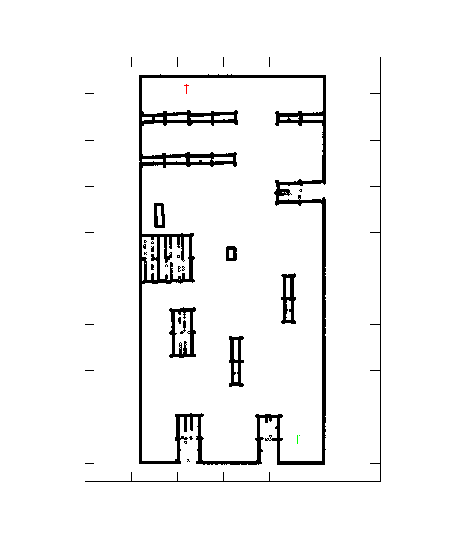
\includegraphics[scale=0.64]{./figures/slides/ch4/warehouse}}%
    \gplfronttext
  \end{picture}%
\endgroup

    \vspace{0.25cm}
    \caption{\small Χάρτης του WAREHOUSE, $\bm{M}_W$}
    \label{fig:02_02_04:map_warehouse}
  \end{subfigure}
  \caption{\small Οι χάρτες των περιβαλλόντων CORRIDOR, $\bm{M}_C$ και
           WAREHOUSE $\bm{M}_W$. Η αρχική στάση του ρομπότ φαίνεται με πράσινο
           χρώμα, ενώ η στάση στόχος του με κόκκινο χρώμα}
\label{fig:02_02_04:maps}
\end{figure}

Για να ελέγξουμε την πρώτη υπόθεση πραγματοποιούμε προσομοιώσεις με τον MCL σε
λειτουργία ανοικτού βρόχου. Συμβολίζοντας με $|\bm{P}_t|$ το μέγεθος του
πληθυσμού σε χρόνο $t>0$, πραγματοποιούμε $N=100$ προσομοιώσεις πλοήγησης για
κάθε μέθοδο επιλογής σωματιδίων, όπως αυτές ορίστηκαν στην ενότητα
\ref{subsection:02_02_03:01}: (α) $100\% \times |\bm{P}_t|$ των σωματιδίων (η
ονομαστική λειτουργία του MCL), (β) υποσυνόλου σωματιδίων $\{i\}$ από το
$\bm{P}_t$ των οποίων το βάρος $w_t^i$ είναι μεγαλύτερο από το μέσο βάρος του
πληθυσμού $\overline{W_t}$ τη χρονική στιγμή $t>0$, (γ) $10\% \times
|\bm{P}_t|$, και (δ) μόνο το σωματίδιο με το μεγαλύτερο βάρος από όλα τα
σωματίδια του $\bm{P}_t$.

Για να ελέγξουμε την τρίτη υπόθεση πραγματοποιούμε $N=100$ προσομοιώσεις
πλοήγησης για κάθε τρόπο ανάδρασης, όπως αυτοί ορίστηκαν στην ενότητα
\ref{subsection:02_02_03:03}, επιλέγοντας όλα τα σωματίδια $|\bm{P}_t|$ για τον
υπολογισμό της τελικής στάσης του MCL, δοκιμάζοντας την απόδοση του σύνθετου
συστήματος (εικόνες \ref{fig:feedback} και \ref{fig:overall_system}) όταν ο
τρόπος ανάδρασης που χρησιμοποιείται είναι (α) κανένας (ανοικτός βρόχος), (β)
soft-$1$ loop-closure, (γ) soft-$50$ loop-closure, και (δ) hard loop-closure.

Για να ελέγξουμε τη δεύτερη υπόθεση παρατηρούμε τα αποτελέσματα όλων των
$4\times100$ προσομοιώσεων που εκτελούνται σε ανοικτό βρόχο και ανά μέθοδο
επιλογής σωματιδίων (η ανάδραση του αποτελέσματος της ευθυγράμμισης μετρήσεων
με σαρώσεις στον MCL εκ των πραγμάτων αλλοιώνει την τυπική επίδοσή του και,
συνεπώς, δεν επιτρέπει την εξαγωγή χρήσιμων συμπερασμάτων για τη συμβολή της
ευθυγράμμισης σαρώσεων σε διάκριση με το συνολικό σύστημα σε κατάσταση κλειστού
βρόχου).

Το κριτήριο στο οποίο στηρίζεται η αξιολόγηση όλων των ελέγχων είναι το πλάτος
του συνολικού σφάλματος στάσης (εξίσωση \ref{eq:pose_error_def}) όπου
$(\hat{x}, \hat{y}, \hat{\theta})$ είναι η εκτιμώμενη στάση του ρομπότ (η οποία
εκτιμάται από τον MCL ή το σύστημα μετά την ευθυγράμμιση σαρώσεων, ανάλογα με
τα συμφραζόμενα), και $(x,y,\theta)$ είναι η πραγματική του στάση, και
επιλέχθηκε ως τέτοιο λόγω της έκφρασης του συνολικού σφάλματος της κατάστασης
του συστήματος και της ικανότητάς του να παρέχει έναν κεντρικό τόπο που
διευκολύνει την άμεση σύγκριση των επιδόσεων της κάθε παραλλαγής του συστήματος
όσον αφορά στην ακρίβεια της στάσης. Για κάθε στάση που εξάγεται από τον MCL σε
μία διαδρομή πλοήγησης (συμβολίζεται με $\hat{\bm{x}}_t$ στο σχήμα
\ref{fig:overall_system}) και το σύστημα μετά την ευθυγράμμιση σαρώσεων
($\hat{\bm{x}}^{\prime}_t$) κατά τη διάρκεια μίας προσομοίωσης, καταγράφουμε τα
σφάλματά τους από την πραγματική στάση του ρομπότ με τη μορφή του συνολικού
σφάλματος. Στη συνέχεια καταγράφουμε το μέσο όρο των σφαλμάτων τους για μία
προσομοίωση, και αναφέρουμε την κατανομή αυτών των τιμών για όλες τις $N = 100$
προσομοιώσεις της ίδιας διαμόρφωσης. Η μονάδα μέτρησης του συνολικού σφάλματος
στάσης είναι $(\text{m}^2+\text{rad}^2)^{1/2}$, και παραλείπεται στα σχήματα
των παρακάτω ενοτήτων για λόγους οικονομίας χώρου.

Σε αντίθεση με τις στάσεις από όπου αξιολογήθηκαν οι επιδόσεις των συστημάτων
των \cite{Rowekamper2012a} και \cite{Vasiljevic2016a} (τα σφάλματα των
συστημάτων τους αξιολογήθηκαν μόνο κοντά σε προκαθορισμένες θέσεις
ενδιαφέροντος του περιβάλλοντος), εμείς αξιολογούμε την επίδοση των ανωτέρω
διαμορφώσεων \textit{κατά μήκος ολόκληρης της διαδρομής} από $\bm{x}_0$ έως
$\bm{x}_G$: αυτό προσφέρει πιο πλήρη εικόνα για την επίδοση των εν λόγω
διαμορφώσεων.

Οι προσομοιώσεις πραγματοποιήθηκαν στο περιβάλλον προσομοίωσης
Gazebo\footnote{\url{http://gazebosim.org/}} μέσω
ROS\footnote{\url{https://www.ros.org/}} στο λειτουργικό σύστημα Linux Ubuntu
16.04, με έναν επεξεργαστή $12$ νημάτων και συχνότητας $4.00$ GHz,
χρησιμοποιώντας έως και $32$ Gb μνήμης RAM. Για την υλοποίηση του MCL με
δειγματοληψία KLD χρησιμοποιήσαμε το ROS πακέτο
\texttt{amcl},\footnote{\url{http://wiki.ros.org/amcl}} το οποίο τροποποιήσαμε
προκειμένου για την επιλογή και εισαγωγή σωματιδίων από και στον πληθυσμό του
φίλτρου. Το σύστημα καταλαμβάνει δύο διεργασίες επεξεργαστή, περίπου 300MB
μνήμης, ενώ η διαδικασία ευθυγράμμισης σαρώσεων χρησιμοποιεί περίπου $5.2\%$
ενός νήματος της CPU.


%%%%%%%%%%%%%%%%%%%%%%%%%%%%%%%%%%%%%%%%%%%%%%%%%%%%%%%%%%%%%%%%%%%%%%%%%%%%%%%%
\subsection{Αποτελέσματα}
\label{subsection:02_02_04:02}

Στα σχήματα \ref{fig:02_02_04:selections}(α') και
\ref{fig:02_02_04:selections}(β') απεικονίζονται οι κατανομές των μέσων
σφαλμάτων στάσης του MCL σε κατάσταση ανοικτού βρόχου και του σύνθετου
συστήματος (σχήμα \ref{fig:overall_system}) ανά διαδρομή του ρομπότ στα
περιβάλλοντα CORRIDOR και WAREHOUSE, ανά μέθοδο επιλογής σωματιδίων. Τα
υποκείμενα σφάλματα θέσης και προσανατολισμού απεικονίζονται στα σχήματα του
παραρτήματος \ref{appendix:02:selection_methods}.


\begin{figure}
  \vspace{2cm}
  \begin{subfigure}{\linewidth}
  \hspace{-1.25cm}
    % GNUPLOT: LaTeX picture with Postscript
\begingroup
  \makeatletter
  \providecommand\color[2][]{%
    \GenericError{(gnuplot) \space\space\space\@spaces}{%
      Package color not loaded in conjunction with
      terminal option `colourtext'%
    }{See the gnuplot documentation for explanation.%
    }{Either use 'blacktext' in gnuplot or load the package
      color.sty in LaTeX.}%
    \renewcommand\color[2][]{}%
  }%
  \providecommand\includegraphics[2][]{%
    \GenericError{(gnuplot) \space\space\space\@spaces}{%
      Package graphicx or graphics not loaded%
    }{See the gnuplot documentation for explanation.%
    }{The gnuplot epslatex terminal needs graphicx.sty or graphics.sty.}%
    \renewcommand\includegraphics[2][]{}%
  }%
  \providecommand\rotatebox[2]{#2}%
  \@ifundefined{ifGPcolor}{%
    \newif\ifGPcolor
    \GPcolorfalse
  }{}%
  \@ifundefined{ifGPblacktext}{%
    \newif\ifGPblacktext
    \GPblacktexttrue
  }{}%
  % define a \g@addto@macro without @ in the name:
  \let\gplgaddtomacro\g@addto@macro
  % define empty templates for all commands taking text:
  \gdef\gplfronttext{}%
  \gdef\gplfronttext{}%
  \makeatother
  \ifGPblacktext
    % no textcolor at all
    \def\colorrgb#1{}%
    \def\colorgray#1{}%
  \else
    % gray or color?
    \ifGPcolor
      \def\colorrgb#1{\color[rgb]{#1}}%
      \def\colorgray#1{\color[gray]{#1}}%
      \expandafter\def\csname LTw\endcsname{\color{white}}%
      \expandafter\def\csname LTb\endcsname{\color{black}}%
      \expandafter\def\csname LTa\endcsname{\color{black}}%
      \expandafter\def\csname LT0\endcsname{\color[rgb]{1,0,0}}%
      \expandafter\def\csname LT1\endcsname{\color[rgb]{0,1,0}}%
      \expandafter\def\csname LT2\endcsname{\color[rgb]{0,0,1}}%
      \expandafter\def\csname LT3\endcsname{\color[rgb]{1,0,1}}%
      \expandafter\def\csname LT4\endcsname{\color[rgb]{0,1,1}}%
      \expandafter\def\csname LT5\endcsname{\color[rgb]{1,1,0}}%
      \expandafter\def\csname LT6\endcsname{\color[rgb]{0,0,0}}%
      \expandafter\def\csname LT7\endcsname{\color[rgb]{1,0.3,0}}%
      \expandafter\def\csname LT8\endcsname{\color[rgb]{0.5,0.5,0.5}}%
    \else
      % gray
      \def\colorrgb#1{\color{black}}%
      \def\colorgray#1{\color[gray]{#1}}%
      \expandafter\def\csname LTw\endcsname{\color{white}}%
      \expandafter\def\csname LTb\endcsname{\color{black}}%
      \expandafter\def\csname LTa\endcsname{\color{black}}%
      \expandafter\def\csname LT0\endcsname{\color{black}}%
      \expandafter\def\csname LT1\endcsname{\color{black}}%
      \expandafter\def\csname LT2\endcsname{\color{black}}%
      \expandafter\def\csname LT3\endcsname{\color{black}}%
      \expandafter\def\csname LT4\endcsname{\color{black}}%
      \expandafter\def\csname LT5\endcsname{\color{black}}%
      \expandafter\def\csname LT6\endcsname{\color{black}}%
      \expandafter\def\csname LT7\endcsname{\color{black}}%
      \expandafter\def\csname LT8\endcsname{\color{black}}%
    \fi
  \fi
  \setlength{\unitlength}{0.0500bp}%
  \begin{picture}(10000.00,4000.00)%
    \gplgaddtomacro\gplfronttext{%
      \colorrgb{0.00,0.00,0.00}%
      \put(1168,440){\makebox(0,0)[r]{\strut{}$0.0$}}%
      \colorrgb{0.00,0.00,0.00}%
      \put(1168,906){\makebox(0,0)[r]{\strut{}$0.01$}}%
      \colorrgb{0.00,0.00,0.00}%
      \put(1168,1371){\makebox(0,0)[r]{\strut{}$0.02$}}%
      \colorrgb{0.00,0.00,0.00}%
      \put(1168,1837){\makebox(0,0)[r]{\strut{}$0.03$}}%
      \colorrgb{0.00,0.00,0.00}%
      \put(1168,2302){\makebox(0,0)[r]{\strut{}$0.04$}}%
      \colorrgb{0.00,0.00,0.00}%
      \put(1168,2768){\makebox(0,0)[r]{\strut{}$0.05$}}%
      \colorrgb{0.00,0.00,0.00}%
      \put(1168,3233){\makebox(0,0)[r]{\strut{}$0.06$}}%
      \colorrgb{0.00,0.00,0.00}%
      \put(1168,3699){\makebox(0,0)[r]{\strut{}$0.07$}}%
      \colorrgb{0.00,0.00,0.00}%
      \put(1625,220){\makebox(0,0){\strut{}$100\%$}}%
      \colorrgb{0.00,0.00,0.00}%
      \put(2493,220){\makebox(0,0){\strut{}$>\overline{W}$}}%
      \colorrgb{0.00,0.00,0.00}%
      \put(3361,220){\makebox(0,0){\strut{}$10\%$}}%
      \colorrgb{0.00,0.00,0.00}%
      \put(4229,220){\makebox(0,0){\strut{}top}}%
      \colorrgb{0.00,0.00,0.00}%
      \put(398,2069){\rotatebox{90}{\makebox(0,0){\strut{}$\overline{\|e\|_{2,i}}$, $i = \{1,2,\dots,N\}$}}}%
      \colorrgb{0.00,0.00,0.00}%
      \put(2927,-110){\makebox(0,0){\strut{}Μέθοδος επιλογής}}%
      \colorrgb{0.00,0.00,0.00}%
      \put(5000,4029){\makebox(0,0){\strut{}Κατανομή μέσων σφαλμάτων εκτίμησης στάσης ανά μέθοδο επιλογής σωματιδίων}}%
    }%
    \gplgaddtomacro\gplfronttext{%
    }%
    \gplgaddtomacro\gplfronttext{%
      \colorrgb{0.00,0.00,0.00}%
      \put(5663,440){\makebox(0,0)[r]{\strut{}$0.010$}}%
      \colorrgb{0.00,0.00,0.00}%
      \put(5663,1092){\makebox(0,0)[r]{\strut{}$0.012$}}%
      \colorrgb{0.00,0.00,0.00}%
      \put(5663,1744){\makebox(0,0)[r]{\strut{}$0.014$}}%
      \colorrgb{0.00,0.00,0.00}%
      \put(5663,2395){\makebox(0,0)[r]{\strut{}$0.016$}}%
      \colorrgb{0.00,0.00,0.00}%
      \put(5663,3047){\makebox(0,0)[r]{\strut{}$0.018$}}%
      \colorrgb{0.00,0.00,0.00}%
      \put(5663,3699){\makebox(0,0)[r]{\strut{}$0.020$}}%
      \colorrgb{0.00,0.00,0.00}%
      \put(6120,220){\makebox(0,0){\strut{}$100\%$}}%
      \colorrgb{0.00,0.00,0.00}%
      \put(6988,220){\makebox(0,0){\strut{}$>\overline{W}$}}%
      \colorrgb{0.00,0.00,0.00}%
      \put(7856,220){\makebox(0,0){\strut{}$10\%$}}%
      \colorrgb{0.00,0.00,0.00}%
      \put(8724,220){\makebox(0,0){\strut{}top}}%
      \colorrgb{0.00,0.00,0.00}%
      \put(7422,-110){\makebox(0,0){\strut{}Μέθοδος επιλογής}}%
      \colorrgb{0.00,0.00,0.00}%
      %\put(7422,4029){\makebox(0,0){\strut{}CORRIDOR pose errors per pose selection method}}%
    }%
    \gplgaddtomacro\gplfronttext{%
    }%
    \gplfronttext
    \put(0,0){\includegraphics{./figures/parts/02/chapters/02/sections/04/corridor_mean_total_errors_per_selection}}%
    \gplfronttext
  \end{picture}%
\endgroup

    \vspace{0.3cm}
    \caption{Περιβάλλον CORRIDOR}
    \label{fig:02_02_04:corridor_selections}
  \end{subfigure}\\
  \begin{subfigure}{\linewidth}\vspace{0.5cm}
    \hspace{-1.25cm}
    % GNUPLOT: LaTeX picture with Postscript
\begingroup
  \makeatletter
  \providecommand\color[2][]{%
    \GenericError{(gnuplot) \space\space\space\@spaces}{%
      Package color not loaded in conjunction with
      terminal option `colourtext'%
    }{See the gnuplot documentation for explanation.%
    }{Either use 'blacktext' in gnuplot or load the package
      color.sty in LaTeX.}%
    \renewcommand\color[2][]{}%
  }%
  \providecommand\includegraphics[2][]{%
    \GenericError{(gnuplot) \space\space\space\@spaces}{%
      Package graphicx or graphics not loaded%
    }{See the gnuplot documentation for explanation.%
    }{The gnuplot epslatex terminal needs graphicx.sty or graphics.sty.}%
    \renewcommand\includegraphics[2][]{}%
  }%
  \providecommand\rotatebox[2]{#2}%
  \@ifundefined{ifGPcolor}{%
    \newif\ifGPcolor
    \GPcolorfalse
  }{}%
  \@ifundefined{ifGPblacktext}{%
    \newif\ifGPblacktext
    \GPblacktexttrue
  }{}%
  % define a \g@addto@macro without @ in the name:
  \let\gplgaddtomacro\g@addto@macro
  % define empty templates for all commands taking text:
  \gdef\gplfronttext{}%
  \gdef\gplfronttext{}%
  \makeatother
  \ifGPblacktext
    % no textcolor at all
    \def\colorrgb#1{}%
    \def\colorgray#1{}%
  \else
    % gray or color?
    \ifGPcolor
      \def\colorrgb#1{\color[rgb]{#1}}%
      \def\colorgray#1{\color[gray]{#1}}%
      \expandafter\def\csname LTw\endcsname{\color{white}}%
      \expandafter\def\csname LTb\endcsname{\color{black}}%
      \expandafter\def\csname LTa\endcsname{\color{black}}%
      \expandafter\def\csname LT0\endcsname{\color[rgb]{1,0,0}}%
      \expandafter\def\csname LT1\endcsname{\color[rgb]{0,1,0}}%
      \expandafter\def\csname LT2\endcsname{\color[rgb]{0,0,1}}%
      \expandafter\def\csname LT3\endcsname{\color[rgb]{1,0,1}}%
      \expandafter\def\csname LT4\endcsname{\color[rgb]{0,1,1}}%
      \expandafter\def\csname LT5\endcsname{\color[rgb]{1,1,0}}%
      \expandafter\def\csname LT6\endcsname{\color[rgb]{0,0,0}}%
      \expandafter\def\csname LT7\endcsname{\color[rgb]{1,0.3,0}}%
      \expandafter\def\csname LT8\endcsname{\color[rgb]{0.5,0.5,0.5}}%
    \else
      % gray
      \def\colorrgb#1{\color{black}}%
      \def\colorgray#1{\color[gray]{#1}}%
      \expandafter\def\csname LTw\endcsname{\color{white}}%
      \expandafter\def\csname LTb\endcsname{\color{black}}%
      \expandafter\def\csname LTa\endcsname{\color{black}}%
      \expandafter\def\csname LT0\endcsname{\color{black}}%
      \expandafter\def\csname LT1\endcsname{\color{black}}%
      \expandafter\def\csname LT2\endcsname{\color{black}}%
      \expandafter\def\csname LT3\endcsname{\color{black}}%
      \expandafter\def\csname LT4\endcsname{\color{black}}%
      \expandafter\def\csname LT5\endcsname{\color{black}}%
      \expandafter\def\csname LT6\endcsname{\color{black}}%
      \expandafter\def\csname LT7\endcsname{\color{black}}%
      \expandafter\def\csname LT8\endcsname{\color{black}}%
    \fi
  \fi
  \setlength{\unitlength}{0.02500bp}%
  \begin{picture}(10000.00,4000.00)%
    \gplgaddtomacro\gplfronttext{%
      \colorrgb{0.00,0.00,0.00}%
      \put(1168,736){\makebox(0,0)[r]{\strut{} \scriptsize $0.03$}}%
      \colorrgb{0.00,0.00,0.00}%
      \put(1168,1107){\makebox(0,0)[r]{\strut{}\scriptsize $0.04$}}%
      \colorrgb{0.00,0.00,0.00}%
      \put(1168,1477){\makebox(0,0)[r]{\strut{}\scriptsize $0.05$}}%
      \colorrgb{0.00,0.00,0.00}%
      \put(1168,1847){\makebox(0,0)[r]{\strut{}\scriptsize $0.06$}}%
      \colorrgb{0.00,0.00,0.00}%
      \put(1168,2218){\makebox(0,0)[r]{\strut{}\scriptsize $0.07$}}%
      \colorrgb{0.00,0.00,0.00}%
      \put(1168,2588){\makebox(0,0)[r]{\strut{}\scriptsize $0.08$}}%
      \colorrgb{0.00,0.00,0.00}%
      \put(1168,2958){\makebox(0,0)[r]{\strut{}\scriptsize $0.09$}}%
      \colorrgb{0.00,0.00,0.00}%
      \put(1168,3329){\makebox(0,0)[r]{\strut{}\scriptsize $0.10$}}%
      \colorrgb{0.00,0.00,0.00}%
      \put(1168,3699){\makebox(0,0)[r]{\strut{}\scriptsize $0.11$}}%
      \colorrgb{0.00,0.00,0.00}%
      \put(1625,220){\makebox(0,0){\strut{}\tiny $100\%$}}%
      \colorrgb{0.00,0.00,0.00}%
      \put(2493,220){\makebox(0,0){\strut{}\tiny $>\hspace{-0.1cm}\overline{W}$}}%
      \colorrgb{0.00,0.00,0.00}%
      \put(3361,220){\makebox(0,0){\strut{}\tiny $10\%$}}%
      \colorrgb{0.00,0.00,0.00}%
      \put(4229,220){\makebox(0,0){\strut{}\tiny top}}%
      \colorrgb{0.00,0.00,0.00}%
      %\put(398,2069){\rotatebox{90}{\makebox(0,0){\strut{}$\overline{\|e\|_{2,i}}$, $i = \{1,2,\dots,N\}$}}}%
      \put(-98,2069){\rotatebox{90}{\makebox(0,0){\strut{} \footnotesize WAREHOUSE}}}%
      %\colorrgb{0.00,0.00,0.00}%
      \put(2927,-210){\makebox(0,0){\strut{}\scriptsize Μέθοδος διαλογής}}%
      %\colorrgb{0.00,0.00,0.00}%
      %\put(2927,4029){\makebox(0,0){\strut{}Κατανομή μέσων σφαλμάτων εκτίμησης στάσης ανά μέθοδο επιλογής σωματιδίων}}%
    }%
    \gplgaddtomacro\gplfronttext{%
    }%
    \gplgaddtomacro\gplfronttext{%
      \colorrgb{0.00,0.00,0.00}%
      \put(5663,440){\makebox(0,0)[r]{\strut{} \scriptsize $0.025$}}%
      \colorrgb{0.00,0.00,0.00}%
      \put(5663,934){\makebox(0,0)[r]{\strut{}\scriptsize $0.030$}}%
      \colorrgb{0.00,0.00,0.00}%
      \put(5663,1428){\makebox(0,0)[r]{\strut{}\scriptsize $0.035$}}%
      \colorrgb{0.00,0.00,0.00}%
      \put(5663,1921){\makebox(0,0)[r]{\strut{}\scriptsize $0.040$}}%
      \colorrgb{0.00,0.00,0.00}%
      \put(5663,2415){\makebox(0,0)[r]{\strut{}\scriptsize $0.045$}}%
      \colorrgb{0.00,0.00,0.00}%
      \put(5663,2909){\makebox(0,0)[r]{\strut{}\scriptsize $0.050$}}%
      \colorrgb{0.00,0.00,0.00}%
      \put(5663,3403){\makebox(0,0)[r]{\strut{}\scriptsize $0.055$}}%
      \colorrgb{0.00,0.00,0.00}%
      \put(6120,220){\makebox(0,0){\strut{}\tiny $100\%$}}%
      \colorrgb{0.00,0.00,0.00}%
      \put(6988,220){\makebox(0,0){\strut{}\tiny $>\hspace{-0.1cm}\overline{W}$}}%
      \colorrgb{0.00,0.00,0.00}%
      \put(7856,220){\makebox(0,0){\strut{}\tiny $10\%$}}%
      \colorrgb{0.00,0.00,0.00}%
      \put(8724,220){\makebox(0,0){\strut{}\tiny top}}%
      \colorrgb{0.00,0.00,0.00}%
      \put(7422,-210){\makebox(0,0){\strut{}\scriptsize Μέθοδος διαλογής}}%
      %\colorrgb{0.00,0.00,0.00}%
      %\put(7422,4029){\makebox(0,0){\strut{}WAREHOUSE pose errors per pose selection method}}%
    }%
    \gplgaddtomacro\gplfronttext{%
    }%
    \put(0,0){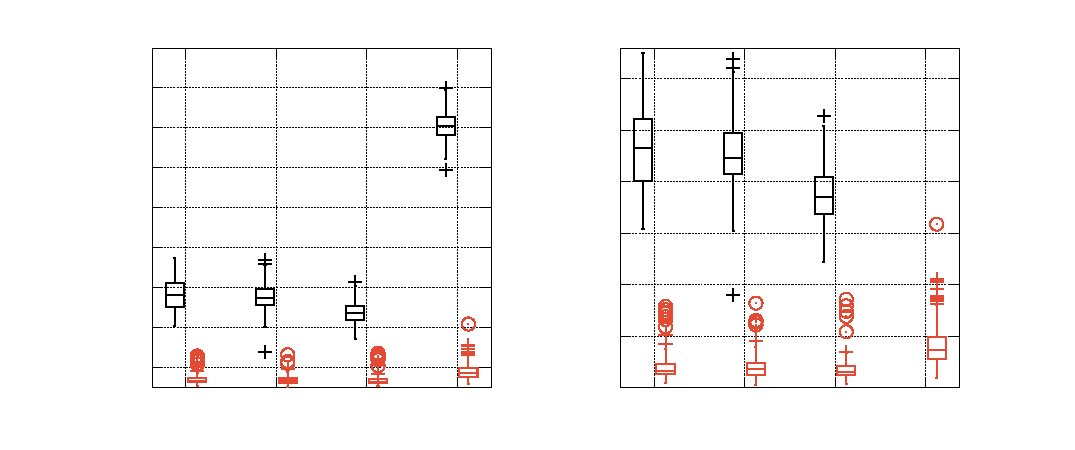
\includegraphics[scale=0.5]{./figures/slides/ch4/experiments/boxplots/warehouse_mean_total_errors_per_selection}}%
    \gplfronttext
  \end{picture}%
\endgroup

    \vspace{0.3cm}
    \caption{Περιβάλλον WAREHOUSE}
    \label{fig:02_02_04:warehouse_selections}
  \end{subfigure}
\caption{\small Η κατανομή του μέσου σφάλματος στάσης ανά διαδρομή πλοήγησης
         για τον MCL σε ανοιχτό βρόχο (στα αριστερά κάθε υποδεικνυόμενης
         μεθόδου επιλογής, με μαύρο χρώμα) και του σύνθετου συστήματος (δεξιά,
         με κόκκινο), σε $N=100$ προσομοιώσεις, ανάλογα με την μέθοδο επιλογής
         πληθυσμού. Το σύμβολο ``$100\%$" υποδηλώνει τη διαμόρφωση του
         συστήματος όπου όλα τα σωματίδια του συνόλου του πληθυσμού επιλέγονται
         κατά τη διαδικασία εξαγωγής της εκτίμησης της στάσης του συστήματος,
         το σύμβολο ``$>\overline{W}$" υποδηλώνει εκείνη της επιλογής των
         σωματιδίων των οποίων το βάρος είναι μεγαλύτερο από το μέσο βάρος του
         πληθυσμού του φίλτρου, το ``$10\%$" εκείνη που μόνο το άνω $10\%$ των
         βαρύτερων σωματιδίων επιλέγονται, και ``top" τη διαμόρφωση όπου
         επιλέγεται μόνο το σωματίδιο με το μεγαλύτερο βάρος μεταξύ όλων των
         σωματιδίων του πληθυσμού}
\label{fig:02_02_04:selections}
\end{figure}

Στα σχήματα \ref{fig:02_02_04:feedbacks}(α') και
\ref{fig:02_02_04:feedbacks}(β') απεικονίζονται οι κατανομές των μέσων
σφαλμάτων στάσης του MCL κλειστού βρόχου και του σύνθετου συστήματος ανά
διαδρομή του ρομπότ στα περιβάλλοντα CORRIDOR και WAREHOUSE, ανά μέθοδο
ανάδρασης. Τα υποκείμενα σφάλματα θέσης και προσανατολισμού απεικονίζονται στα
σχήματα του παραρτήματος \ref{appendix:02:feedback_methods}.

\begin{figure}
  \vspace{2cm}
  \begin{subfigure}{\linewidth}
  \hspace{-1.25cm}
    \definecolor{r}{RGB}{227,74,51}
\definecolor{k}{RGB}{0,0,0}
% GNUPLOT: LaTeX picture with Postscript
\begingroup
  \makeatletter
  \providecommand\color[2][]{%
    \GenericError{(gnuplot) \space\space\space\@spaces}{%
      Package color not loaded in conjunction with
      terminal option `colourtext'%
    }{See the gnuplot documentation for explanation.%
    }{Either use 'blacktext' in gnuplot or load the package
      color.sty in LaTeX.}%
    \renewcommand\color[2][]{}%
  }%
  \providecommand\includegraphics[2][]{%
    \GenericError{(gnuplot) \space\space\space\@spaces}{%
      Package graphicx or graphics not loaded%
    }{See the gnuplot documentation for explanation.%
    }{The gnuplot epslatex terminal needs graphicx.sty or graphics.sty.}%
    \renewcommand\includegraphics[2][]{}%
  }%
  \providecommand\rotatebox[2]{#2}%
  \@ifundefined{ifGPcolor}{%
    \newif\ifGPcolor
    \GPcolorfalse
  }{}%
  \@ifundefined{ifGPblacktext}{%
    \newif\ifGPblacktext
    \GPblacktexttrue
  }{}%
  % define a \g@addto@macro without @ in the name:
  \let\gplgaddtomacro\g@addto@macro
  % define empty templates for all commands taking text:
  \gdef\gplfronttext{}%
  \gdef\gplfronttext{}%
  \makeatother
  \ifGPblacktext
    % no textcolor at all
    \def\colorrgb#1{}%
    \def\colorgray#1{}%
  \else
    % gray or color?
    \ifGPcolor
      \def\colorrgb#1{\color[rgb]{#1}}%
      \def\colorgray#1{\color[gray]{#1}}%
      \expandafter\def\csname LTw\endcsname{\color{white}}%
      \expandafter\def\csname LTb\endcsname{\color{black}}%
      \expandafter\def\csname LTa\endcsname{\color{black}}%
      \expandafter\def\csname LT0\endcsname{\color[rgb]{1,0,0}}%
      \expandafter\def\csname LT1\endcsname{\color[rgb]{0,1,0}}%
      \expandafter\def\csname LT2\endcsname{\color[rgb]{0,0,1}}%
      \expandafter\def\csname LT3\endcsname{\color[rgb]{1,0,1}}%
      \expandafter\def\csname LT4\endcsname{\color[rgb]{0,1,1}}%
      \expandafter\def\csname LT5\endcsname{\color[rgb]{1,1,0}}%
      \expandafter\def\csname LT6\endcsname{\color[rgb]{0,0,0}}%
      \expandafter\def\csname LT7\endcsname{\color[rgb]{1,0.3,0}}%
      \expandafter\def\csname LT8\endcsname{\color[rgb]{0.5,0.5,0.5}}%
    \else
      % gray
      \def\colorrgb#1{\color{black}}%
      \def\colorgray#1{\color[gray]{#1}}%
      \expandafter\def\csname LTw\endcsname{\color{white}}%
      \expandafter\def\csname LTb\endcsname{\color{black}}%
      \expandafter\def\csname LTa\endcsname{\color{black}}%
      \expandafter\def\csname LT0\endcsname{\color{black}}%
      \expandafter\def\csname LT1\endcsname{\color{black}}%
      \expandafter\def\csname LT2\endcsname{\color{black}}%
      \expandafter\def\csname LT3\endcsname{\color{black}}%
      \expandafter\def\csname LT4\endcsname{\color{black}}%
      \expandafter\def\csname LT5\endcsname{\color{black}}%
      \expandafter\def\csname LT6\endcsname{\color{black}}%
      \expandafter\def\csname LT7\endcsname{\color{black}}%
      \expandafter\def\csname LT8\endcsname{\color{black}}%
    \fi
  \fi
  \setlength{\unitlength}{0.0500bp}%
  \begin{picture}(10000.00,4000.00)%
    \gplgaddtomacro\gplfronttext{%
      \colorrgb{0.00,0.00,0.00}%
      \put(1168,440){\makebox(0,0)[r]{\strut{}$0.0$}}%
      \colorrgb{0.00,0.00,0.00}%
      \put(1168,983){\makebox(0,0)[r]{\strut{}$0.01$}}%
      \colorrgb{0.00,0.00,0.00}%
      \put(1168,1526){\makebox(0,0)[r]{\strut{}$0.02$}}%
      \colorrgb{0.00,0.00,0.00}%
      \put(1168,2070){\makebox(0,0)[r]{\strut{}$0.03$}}%
      \colorrgb{0.00,0.00,0.00}%
      \put(1168,2613){\makebox(0,0)[r]{\strut{}$0.04$}}%
      \colorrgb{0.00,0.00,0.00}%
      \put(1168,3156){\makebox(0,0)[r]{\strut{}$0.05$}}%
      \colorrgb{0.00,0.00,0.00}%
      \put(1168,3699){\makebox(0,0)[r]{\strut{}$0.06$}}%
      \colorrgb{0.00,0.00,0.00}%
      \put(1625,220){\makebox(0,0){\strut{}open}}%
      \colorrgb{0.00,0.00,0.00}%
      \put(2493,220){\makebox(0,0){\strut{}soft-$1$}}%
      \colorrgb{0.00,0.00,0.00}%
      \put(3361,220){\makebox(0,0){\strut{}soft-$50$}}%
      \colorrgb{0.00,0.00,0.00}%
      \put(4229,220){\makebox(0,0){\strut{}hard}}%
      \colorrgb{0.00,0.00,0.00}%
      \put(398,2069){\rotatebox{90}{\makebox(0,0){\strut{}$\overline{\|\bm{e}\|_{2,i}}$, $i = \{1,2,\dots,N\}$}}}%
      \colorrgb{0.00,0.00,0.00}%
      \put(2927,-110){\makebox(0,0){\strut{}Μέθοδος ανάδρασης}}%
      \colorrgb{0.00,0.00,0.00}%
      \put(5000,4729){\makebox(0,0){\strut{}Κατανομή μέσων σφαλμάτων εκτίμησης στάσης ανά μέθοδο ανάδρασης}}%
      \put(2900,3900){\makebox(0,0){\strut{}Πλήρης άποψη}}%
      \put(7350,3900){\makebox(0,0){\strut{}Εστιασμένη άποψη}}%
      \put(4100,4329){\makebox(0,0){\strut{}{\color{k}{\rule[0.6mm]{0.5cm}{0.5mm}}} $\|\bm{e}(\hat{x}_t,x_t)\|_2$}}
      \put(5900,4329){\makebox(0,0){\strut{}{\color{r}{\rule[0.6mm]{0.5cm}{0.5mm}}} $\|\bm{e}(\hat{x}_t^\prime,x_t)\|_2$}}
      }%
    \gplgaddtomacro\gplfronttext{%
    }%
    \gplgaddtomacro\gplfronttext{%
      \colorrgb{0.00,0.00,0.00}%
      \put(5663,440){\makebox(0,0)[r]{\strut{}$0.011$}}%
      \colorrgb{0.00,0.00,0.00}%
      \put(5663,2070){\makebox(0,0)[r]{\strut{}$0.0115$}}%
      \colorrgb{0.00,0.00,0.00}%
      \put(5663,3699){\makebox(0,0)[r]{\strut{}$0.012$}}%
      \colorrgb{0.00,0.00,0.00}%
      \put(6120,220){\makebox(0,0){\strut{}open}}%
      \colorrgb{0.00,0.00,0.00}%
      \put(6988,220){\makebox(0,0){\strut{}soft-$1$}}%
      \colorrgb{0.00,0.00,0.00}%
      \put(7856,220){\makebox(0,0){\strut{}soft-$50$}}%
      \colorrgb{0.00,0.00,0.00}%
      \put(8724,220){\makebox(0,0){\strut{}hard}}%
      \colorrgb{0.00,0.00,0.00}%
      \put(7422,-110){\makebox(0,0){\strut{}Μέθοδος ανάδρασης}}%
      \colorrgb{0.00,0.00,0.00}%
    }%
    \gplgaddtomacro\gplfronttext{%
    }%
    \gplfronttext
    \put(0,0){\includegraphics{./figures/parts/02/chapters/02/sections/04/corridor_mean_total_errors_per_feedback}}%
    \gplfronttext
  \end{picture}%
\endgroup

    \vspace{0.3cm}
    \caption{Περιβάλλον CORRIDOR}
    \label{}
  \end{subfigure}\\
  \begin{subfigure}{\linewidth}\vspace{0.5cm}
    \hspace{-1.25cm}
    \input{./figures/parts/02/chapters/02/sections/04/warehouse_mean_total_errors_per_feedback.tex}
    \vspace{0.3cm}
    \caption{Περιβάλλον WAREHOUSE}
    \label{}
    \end{subfigure}
\caption{\small Η κατανομή του μέσου σφάλματος στάσης ανά διαδρομή πλοήγησης
         για τον MCL (στα αριστερά κάθε υποδεικνυόμενης μεθόδου ανάδρασης, με
         μαύρο χρώμα) και του σύνθετου συστήματος (δεξιά, με κόκκινο) σε
         $N=100$ προσομοιώσεις, ανάλογα με τη μέθοδο ανατροφοδότησης του
         αποτελέσματος της ευθυγράμμισης μετρήσεων με σαρώσεις χάρτη. Η φράση
         ``open" είναι συντομογραφία για την έλλειψη ανάδρασης (ανοιχτός
         βρόχος), η φράση ``soft-$1$" για τη διαμόρφωση όπου η έξοδος του
         συνολικού συστήματος επιστρέφει στο φίλτρο σωματιδίων με τη μορφή ενός
         σωματιδίου, ``soft-$50$" για την περίπτωση που επιστρέφει με τη μορφή
         τόσων σωματιδίων όσα το μισό μέγεθος του πληθυσμού, και ``hard" για τη
         διαμόρφωση όπου το φίλτρο σωματιδίων αρχικοποιείται γύρω από τη στάση
         που υπολογίζεται μετά τη διαδικασία ευθυγράμμισης}
\label{fig:02_02_04:feedbacks}
\end{figure}


%%%%%%%%%%%%%%%%%%%%%%%%%%%%%%%%%%%%%%%%%%%%%%%%%%%%%%%%%%%%%%%%%%%%%%%%%%%%%%%%
\subsection{Αξιολόγηση μεθόδων επιλογής σωματιδίων}
\label{subsection:02_02_04:03}

Όσον αφορά στις μεθόδους επιλογής σωματιδίων εστιάζουμε στα σφάλματα του MCL
ανοικτού βρόχου (τα boxplots μαύρου χρώματος του σχήματος
\ref{fig:02_02_04:selections}) διότι η επίδοση της κάθε μεθόδου επιλογής
σωματιδίων μπορεί να διακριθεί με σαφήνεια, καθώς δεν αλλοιώνεται από την
ανατροφοδότηση ή την επίδοση της ευθυγράμμισης σαρώσεων. Στρέφοντας την προσοχή
μας στα σχήματα διακρίνουμε καταρχάς ότι επιλέγοντας σωματίδια των οποίων το
βάρος είναι μεγαλύτερο από το μέσο βάρους του πληθυσμού κατά τη στιγμή της
επιλογής τους έχει ως αποτέλεσμα χαμηλότερα σφάλματα στάσης σε σύγκριση με την
επιλογή όλων των σωματιδίων, και στα δύο προσομοιωμένα περιβάλλοντα. Το
αποτέλεσμα αυτό είναι διαισθητικά λογικό, δεδομένου ότι αναμένει κανείς ότι τα
σωματίδια που συμβάλλουν στη συνολική στάση με βάρος μικρότερο από το μέσο
βάρος του πληθυσμού έχουν συνολικά αρνητική συνεισφορά στην ακρίβεια της
στάσης, η οποία, όπως φαίνεται από τα δεδομένα, είναι σχεδόν αμελητέα.
Επιπλέον, σε αντίθεση με τις άλλες δύο πρακτικές επιλογής σωματιδίων που
παρουσιάστηκαν, αυτή είναι η λιγότερο καταστροφική, αφού αγκυροβολεί την
πρακτική απόρριψης σωματιδίων στη μεταβαλλόμενη μέση τιμή βάρους του πληθυσμού
και, επομένως, επιλέγει σωματίδια των οποίων ο αριθμός είναι δυναμικός, αντί να
την βασίζει στον αριθμό των βαρύτερων σωματιδίων και να επιλέγει σωματίδια των
οποίων ο αριθμός είναι σταθερός.

Τούτου λεχθέντος, η επιλογή του $10\%$ των βαρύτερων σωματιδίων σε κάθε
επανάληψη υπερτερεί της επιλογής σωματιδίων των οποίων το βάρος είναι
μεγαλύτερο του μέσου βάρους του πληθυσμού. Για την ακρίβεια, το μοτίβο της
ελάττωσης του σφάλματος στάσης και στα δυό περιβάλλοντα είναι το ίδιο: η
επιλογή του $10\%$ των βαρύτερων σωματιδίων σε κάθε επανάληψη υπερτερεί της
επιλογής σωματιδίων των οποίων το βάρος είναι μεγαλύτερο από το μέσο βάρος του
πληθυσμού κατά τη στιγμή της επιλογής τους, η οποία, με τη σειρά της, υπερτερεί
της τυπικής επιλογής όλων των σωματιδίων.

Αυτό που είναι αντιδιαισθητικό είναι τα αυξημένα σφάλματα στάσης όταν
επιλέγεται μόνο το βαρύτερο σωματίδιο ως εκτίμηση της στάσης του φίλτρου, και
στα δύο περιβάλλοντα: αυτό που θα περίμενε κανείς είναι ότι το σωματίδιο με το
μεγαλύτερο βάρος, δηλαδή το σωματίδιο του οποίου η εκτίμηση στάσης εξηγεί
καλύτερα από όλα τα υπόλοιπα σωματίδια του πληθυσμού τις εισερχόμενες
μετρήσεις, και το οποίο είναι τότε, θεωρητικά, η καλύτερη εκτίμηση του
φίλτρου---θα περίμενε κανείς ότι θα παρουσίαζε το χαμηλότερο σφάλμα στάσης.
Στην πραγματικότητα όμως, σύμφωνα με τα δεδομένα αποτελέσματα, το βαρύτερο
σωματίδιο είναι λιγότερο ακριβές από τη συλλογική εκτίμηση του φίλτρου. Αυτή η
ασυμφωνία υποδηλώνει ότι ίσως υπάρχει ένα κατώφλι από το οποίο και άνω
επιβεβαιώνεται η ελεγχόμενη υπόθεση\footnote{Αν το βαρύτερο σωματίδιο εμφανίζει
υψηλότερο σφάλμα από το συλλογικό πληθυσμό, αλλά το $10\%$ των βαρύτερων
σωματιδίων εμφανίζει χαμηλότερο σφάλμα από τον πληθυσμό, τότε, επί της αρχής,
υπάρχει ένα κατώφλι αριθμού βαρύτερων σωματιδίων των οποίων ο σταθμισμένος
μέσος όρος εκτίμησης εμφανίζει την ίδια ακρίβεια με εκείνον του πληθυσμού, κατ'
αναλογία με το θεώρημα Bolzano.} και ότι, δεδομένων των αποδεικτικών στοιχείων,
το σωματίδιο που υπολογίζει καλύτερα τις εισερχόμενες μετρήσεις δεν κατέχει την
καλύτερη αξιοπιστία σε σύγκριση με εκείνη του πληθυσμού ως συλλογικότητα. Αυτή
είναι ουσιαστικά η θεωρία πίσω από τη μη απόρριψη σωματιδίων με χαμηλό βάρος,
δεδομένου ότι το καλύτερο σωματίδιο μπορεί να είναι βέλτιστο τοπικά (για τις
τελευταίες επαναλήψεις) αλλά όχι σε καθολικό επίπεδο. Αυτή η συμπεριφορά μας
ωθεί να θεωρήσουμε ότι ένα φίλτρο σωματιδίων δεν μπορεί να θεωρηθεί ως μια
συνάθροιση ξεχωριστών εκτιμήσεων, αλλά μάλλον ως μια κατακερματισμένη εκτίμηση,
όπου κανένα
κέρμα\footnote{\href{https://www.greek-language.gr/digitalResources/ancient_greek/tools/liddell-scott/search.html?lq=\%CE\%BA\%CE\%AD\%CF\%81\%CE\%BC\%CE\%B1}
{\textbf{κέρμα, -ατος, τό (κείρω)}, 1.  τεμάχιο· απ' όπου, μικρό νόμισμα,
οβολός.}} δεν μπορεί να υποκαταστήσει το σύνολο χωρίς ανεπανόρθωτη απώλεια
πληροφορίας και μείωση της ποιότητας της
εκτίμησης.\footnote{\href{https://bit.ly/3Hw9T12}{[...] πάντων γὰρ οσα πλείω
μέρη εχει καὶ μὴ ἔστιν οἷον σωρὸς τὸ πᾶν ἀλλ' ἔστι τι τὸ ὅλον παρὰ τὰ μόρια
[...]. Αριστοτέλης, Μετά τα Φυσικά}} Αυτή η αντιστροφή στην ποιότητα της
εκτίμησης μπορεί να αποδοθεί στην περιθωριοποίηση της πληροφορίας που φέρει ο
υπόλοιπος πληθυσμός, συμπεριλαμβανομένης της τυχαιότητας που εισάγει η
δειγματοληψία KLD καθώς δημιουργεί νέα σωματίδια.

Αυτή η συμπεριφορά δεν υποσκάπτει τη μέθοδο επιλογής των κορυφαίων $10\%$
βαρύτερων σωματιδίων, καθώς, αν και υποδεικνύει την πιθανότητα ότι θα είχε την
ίδια τύχη αν το μέγιστο μέγεθος του πληθυσμού ήταν σημαντικά μικρότερο, η
αξιοπιστία του φίλτρου θα διακυβευόταν επίσης με ένα τόσο χαμηλό μέγιστο
μέγεθος---και εν πάση περιπτώσει ένα χαμηλό μέγεθος πληθυσμού μειονεκτεί όσον
αφορά τόσο στην ποιότητα της εκτίμησης του συνολικού πληθυσμού (η εξάντληση των
σωματιδίων είναι ο κίνδυνος εδώ) όσο και σε ό,τι αφορά εκείνη ενός υποσυνόλου
του.


%%%%%%%%%%%%%%%%%%%%%%%%%%%%%%%%%%%%%%%%%%%%%%%%%%%%%%%%%%%%%%%%%%%%%%%%%%%%%%%%
\subsection{Αξιολόγηση ευθυγράμμισης μετρήσεων με σαρώσεις χάρτη}
\label{subsection:02_02_04:04}

Όσον αφορά στη συγκριτική επίδοση της ευθυγράμμισης μετρήσεων lidar με σαρώσεις
χάρτη σε σχέση με την επίδοση του φίλτρου σωματιδίων, εστιάζουμε στα σφάλματα
του συνολικού συστήματος (τα boxplots κόκκινου χρώματος του σχήματος
\ref{fig:02_02_04:selections}), και τα μεγέθη τους σε σχέση με τα σφάλματα
στάσης του MCL σε κατάσταση ανοικτού βρόχου (τα boxplots μαύρου χρώματος του
ιδίου σχήματος).

Εν γένει η στάση που εξάγεται μέσω της ευθυγράμμισης μετρήσεων με σαρώσεις
είναι λιγότερο εσφαλμένη από εκείνη που εξάγεται από τον MCL για όλες τις
διαμορφώσεις μεθόδων επιλογής σωματιδίων σε ανοικτό βρόχο, με τη μείωση του
σφάλματος να κυμαίνεται από μερικά χιλιοστά (στην περίπτωση του απλού χάρτη
CORRIDOR) έως μερικά εκατοστά (στην περίπτωση του πιο σύνθετου χάρτη
WAREHOUSE).

%%%%%%%%%%%%%%%%%%%%%%%%%%%%%%%%%%%%%%%%%%%%%%%%%%%%%%%%%%%%%%%%%%%%%%%%%%%%%%%%
\subsection{Αξιολόγηση μεθόδων ανάδρασης}
\label{subsection:02_02_04:05}

Όσον αφορά στις μεθόδους ανάδρασης εστιάζουμε στα σφάλματα του MCL (τα
boxplots μαύρου χρώματος του σχήματος \ref{fig:02_02_04:feedbacks}). Η διαφορά
της επίδοσης μεταξύ της μεθόδου soft-$50$ loop-closure και του MCL σε κατάσταση
ανοιχτού βρόχου: τα σφάλματα στάσης της πρώτης είναι περίπου $32\%$ χαμηλότερα
από εκείνα του MCL στο περιβάλλον CORRIDOR, και περίπου $89\%$ χαμηλότερα στο
περιβάλλον WAREHOUSE. Η διαφορά της επίδοσης της μεθόδου κλεισίματος βρόχου
soft-$50$ loop-closure σε σύγκριση με εκείνη της soft-$1$ είναι αμελητέα στο
απλό περιβάλλον CORRIDOR, ωστόσο, στο σύνθετο περιβάλλον WAREHOUSE τα σφάλματα
της πρώτης μεθόδου είναι μειωμένα κατά σχεδόν $121\%$ έναντι της δεύτερης.

Κατά τη σύγκριση της διαφοράς της επίδοσης των μεθόδων ανατροφοδότησης
soft-$50$ και hard-loop-closure παρατηρούμε ότι στο περιβάλλον CORRIDOR είναι
συγκρίσιμες, με την πρώτη να υπερέχει της δεύτερης συνολικά. Αυτό που είναι
εντυπωσιακό όμως είναι η διαφορά στις επιδόσεις τους στο περιβάλλον WAREHOUSE
(σχήμα \ref{fig:02_02_04:feedbacks}(β'), αριστερά): κατά το κλείσιμο του βρόχου
με τη μέθοδο hard-loop-closure το σύστημα δεν μπόρεσε να ανακάμψει από σοβαρά
σφάλματα εκτίμησης στάσης μετά την εφαρμογή του αποτελέσματος της ευθυγράμμισης
μετρήσεων με σαρώσεις χάρτη, καθώς ο πληθυσμός του φίλτρου αρχικοποιείται εκ
νέου σε κάθε στάση που εξάγεται από την τελευταία, ανεξάρτητα από την ακρίβειά
της. Αντιθέτως, υποθέτοντας ότι, στατιστικά, ένας αριθμός παρόμοιων σφαλμάτων
προέκυψε στα πειράματα όπου χρησιμοποιήθηκε το κλείσιμο του βρόχου soft-$50$,
αυτή η συμπεριφορά απουσίαζε. Ο λόγος για αυτή την εύρωστη συμπεριφορά είναι
ο ακόλουθος: μετά την εισαγωγή του αποτελέσματος της ευθυγράμμισης μετρήσεων με
σαρώσεις στον πληθυσμό του φίλτρου σωματιδίων ως ένας αριθμός νέων υποθέσεων,
το φίλτρο αποδίδει εσωτερικά ένα βάρος σε κάθε μία από αυτές (ενότητα
\ref{subsec:01_01_02_3}), και, εάν οι στάσεις αυτών των σωματιδίων είναι σοβαρά
λανθασμένες, αυτό αντικατοπτρίζεται στις τιμές των βαρών τους, καθώς αυτές οι
στάσεις εξηγούν τις εισερχόμενες μετρήσεις μάλλον ανεπαρκώς. Δεδομένου ότι η
στάση εξόδου του MCL είναι ο σταθμισμένος μέσος όρος όλων των εκτιμήσεων του
πληθυσμού, αυτά τα σωματίδια συμμετέχουν στην τελική ψηφοφορία σε ελάχιστο
ποσοστό και, επομένως, η εκτίμηση του φίλτρου είναι σε μεγάλο βαθμό αδιατάρακτη
από τις χαμηλής ποιότητας υποθέσεις, παρουσιάζοντας την ίδια εύρωστη
συμπεριφορά με τον τυπικό MCL. Το πλεονέκτημα της ενσωμάτωσης της
δειγματοληψίας KLD στον MCL είναι ότι τα σωματίδια των οποίων το βάρος είναι
ελάχιστο απορρίπτονται στη συνέχεια από τον πληθυσμό, μην αφήνοντάς τους χώρο
να επηρεάσουν την συνοχή της εσωτερικής του εκτίμησης στις επόμενες
επαναλήψεις. Αντιθέτως, κατά την ανατροφοδότηση του αποτελέσματος της
ευθυγράμμισης μετρήσεων με σαρώσεις χάρτη μέσω της μεθόδου ανάδρασης
hard-loop-closure, το σύνολο του πληθυσμού των σωματιδίων του φίλτρου
μεταφέρεται και διασπείρεται γύρω από την εσφαλμένη στάση, την οποία το φίλτρο
εσφαλμένα θεωρεί ως μία στη γειτονιά της πραγματικής στάσης του ρομπότ.  Στη
συνέχεια, η μέθοδος MCL αδυνατεί να γεφυρώσει μεγάλα κενά είτε στη θέση είτε
στον προσανατολισμό ανάμεσα σε διαδοχικές εκτελέσεις, με αποτέλεσμα τον κίνδυνο
της ακεραιότητας του ρομπότ, του περιβάλλοντός του, και, εν πάση περιπτώσει,
την αδυναμία συνέχισης της πλοήγησής του, και συνεπώς της αποστολής του.
